\chapter{\label{cha:transquest}TransQuest: STS Architectures for QE}

\section{Introduction}
\cite{conneau-etal-2020-unsupervised} 
\section{Methodology}



\begin{figure}[!ht]
	\centering
	\begin{subfigure}[b]{10cm}
		\centering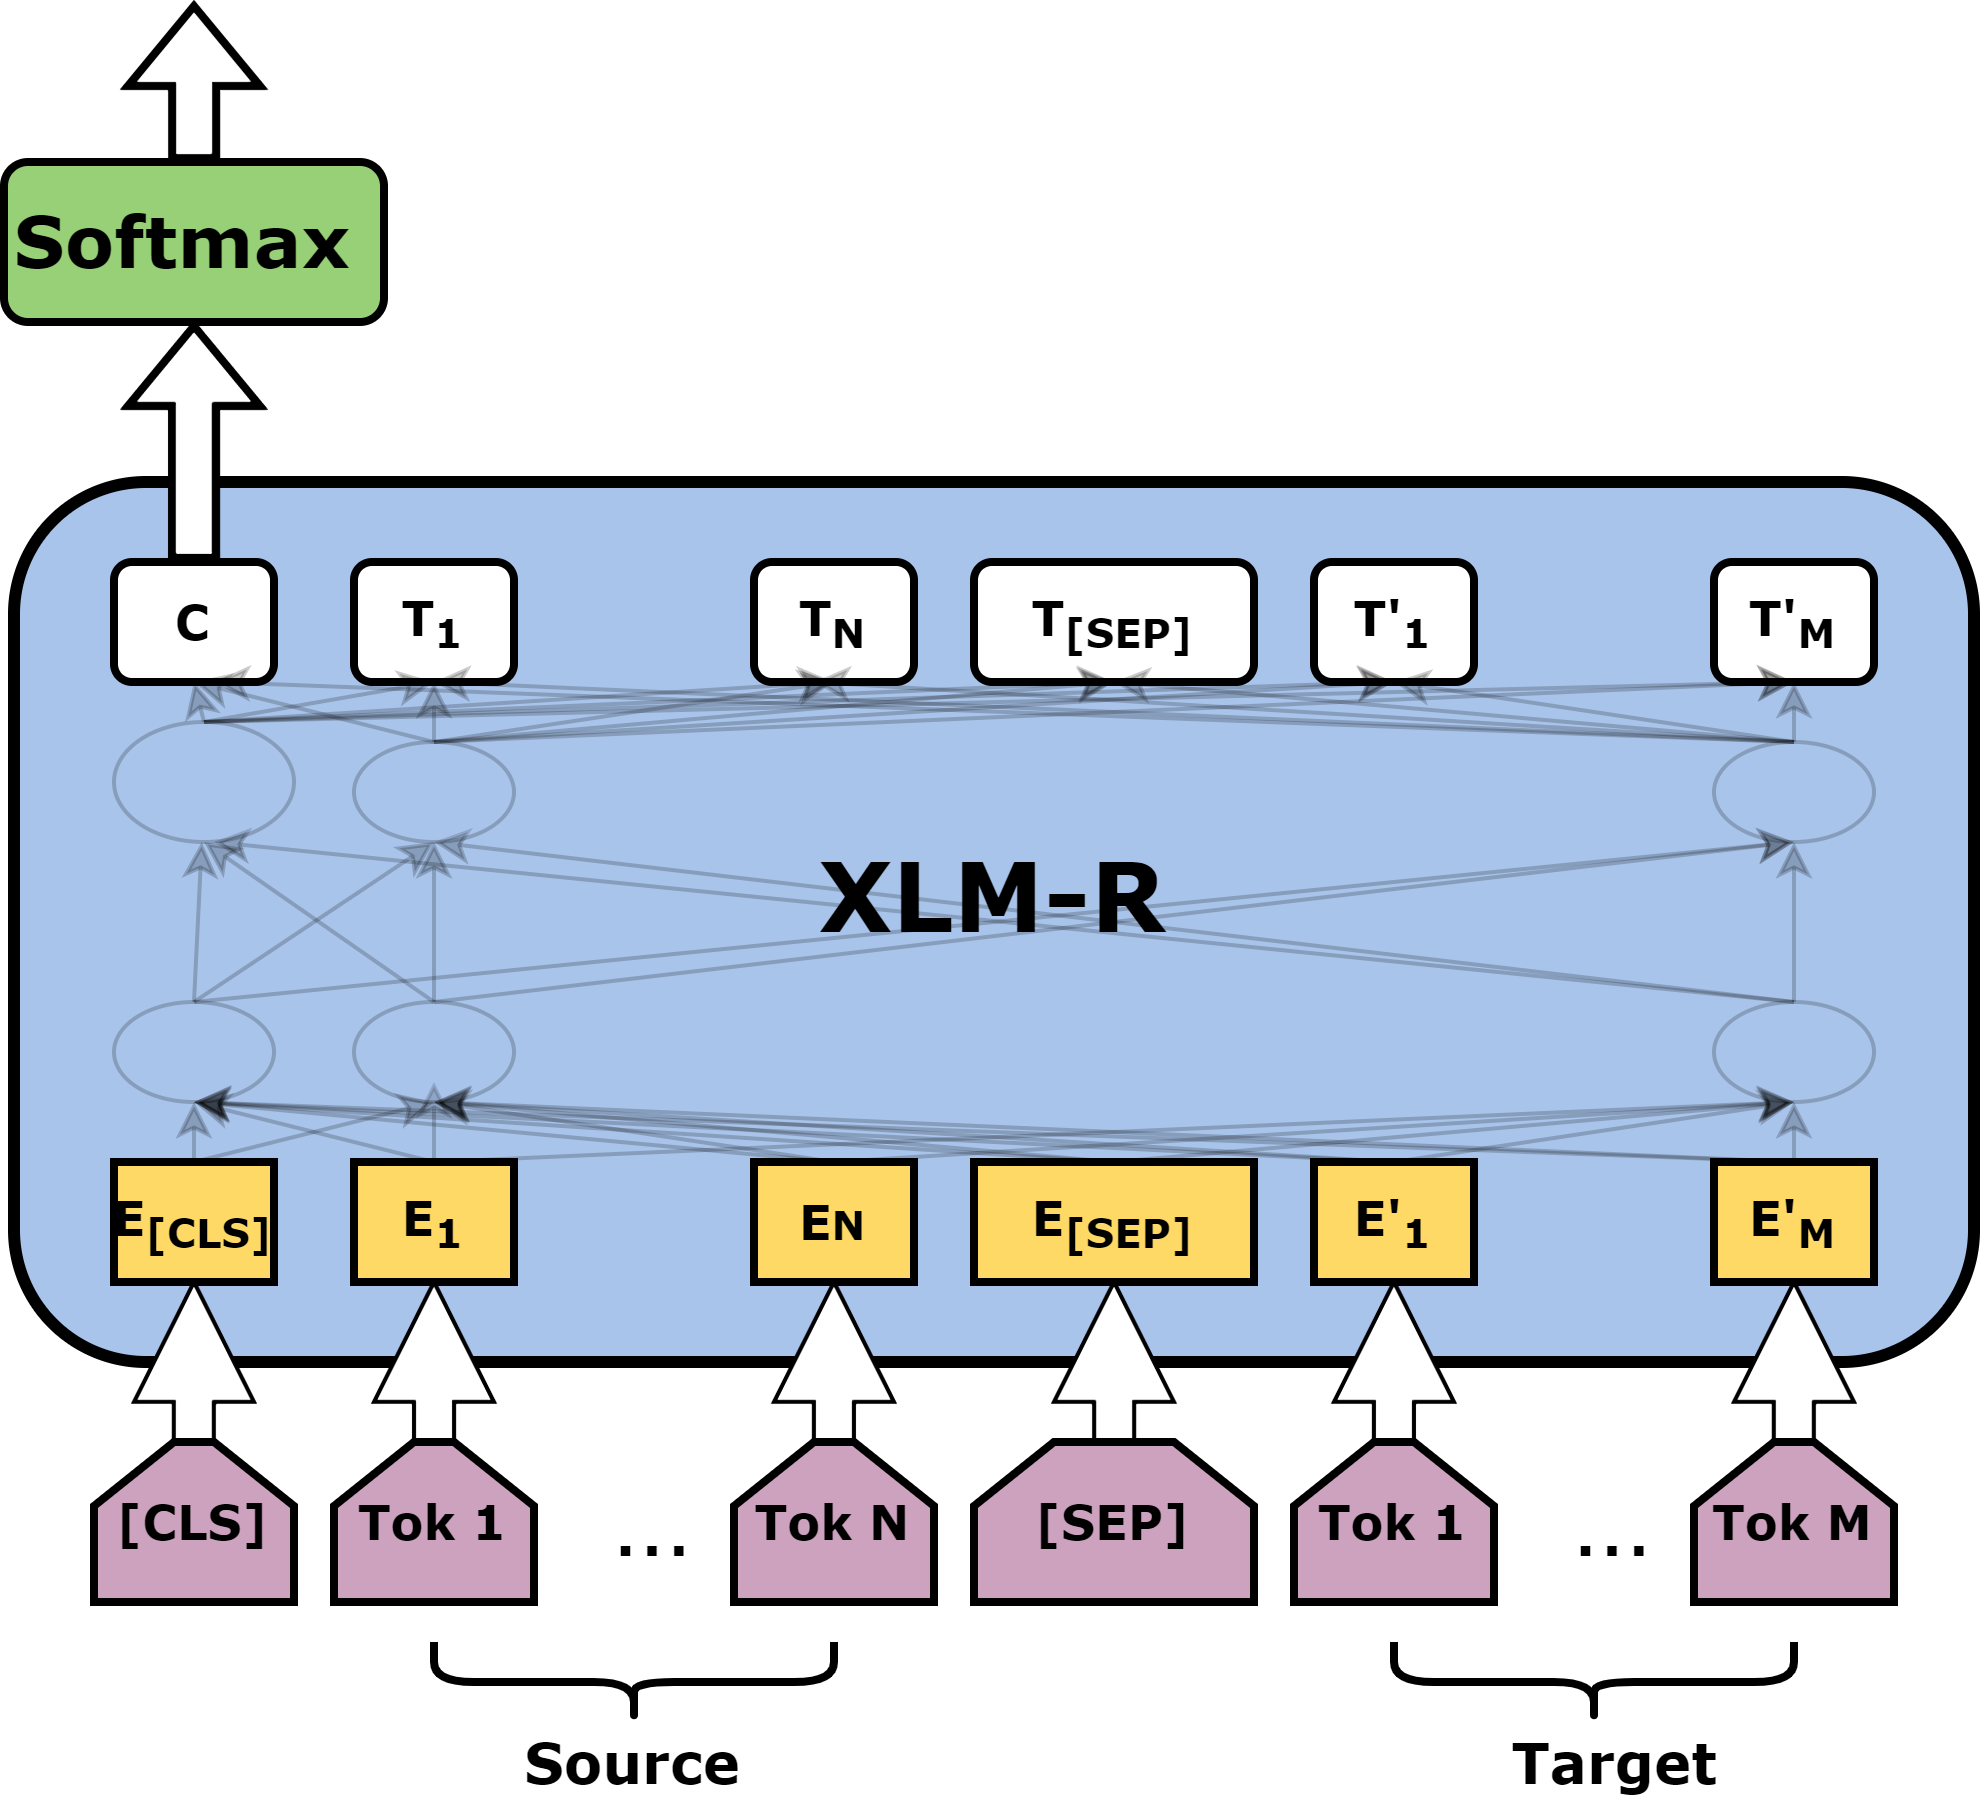
\includegraphics[width=8cm]{figures/translation_quality_estimation/TransQuest.png}
		\caption{\textit{MonoTransQuest} architecture}
		\label{fig:monotransquest}
	\end{subfigure}
	\begin{subfigure}[b]{10cm}
		\centering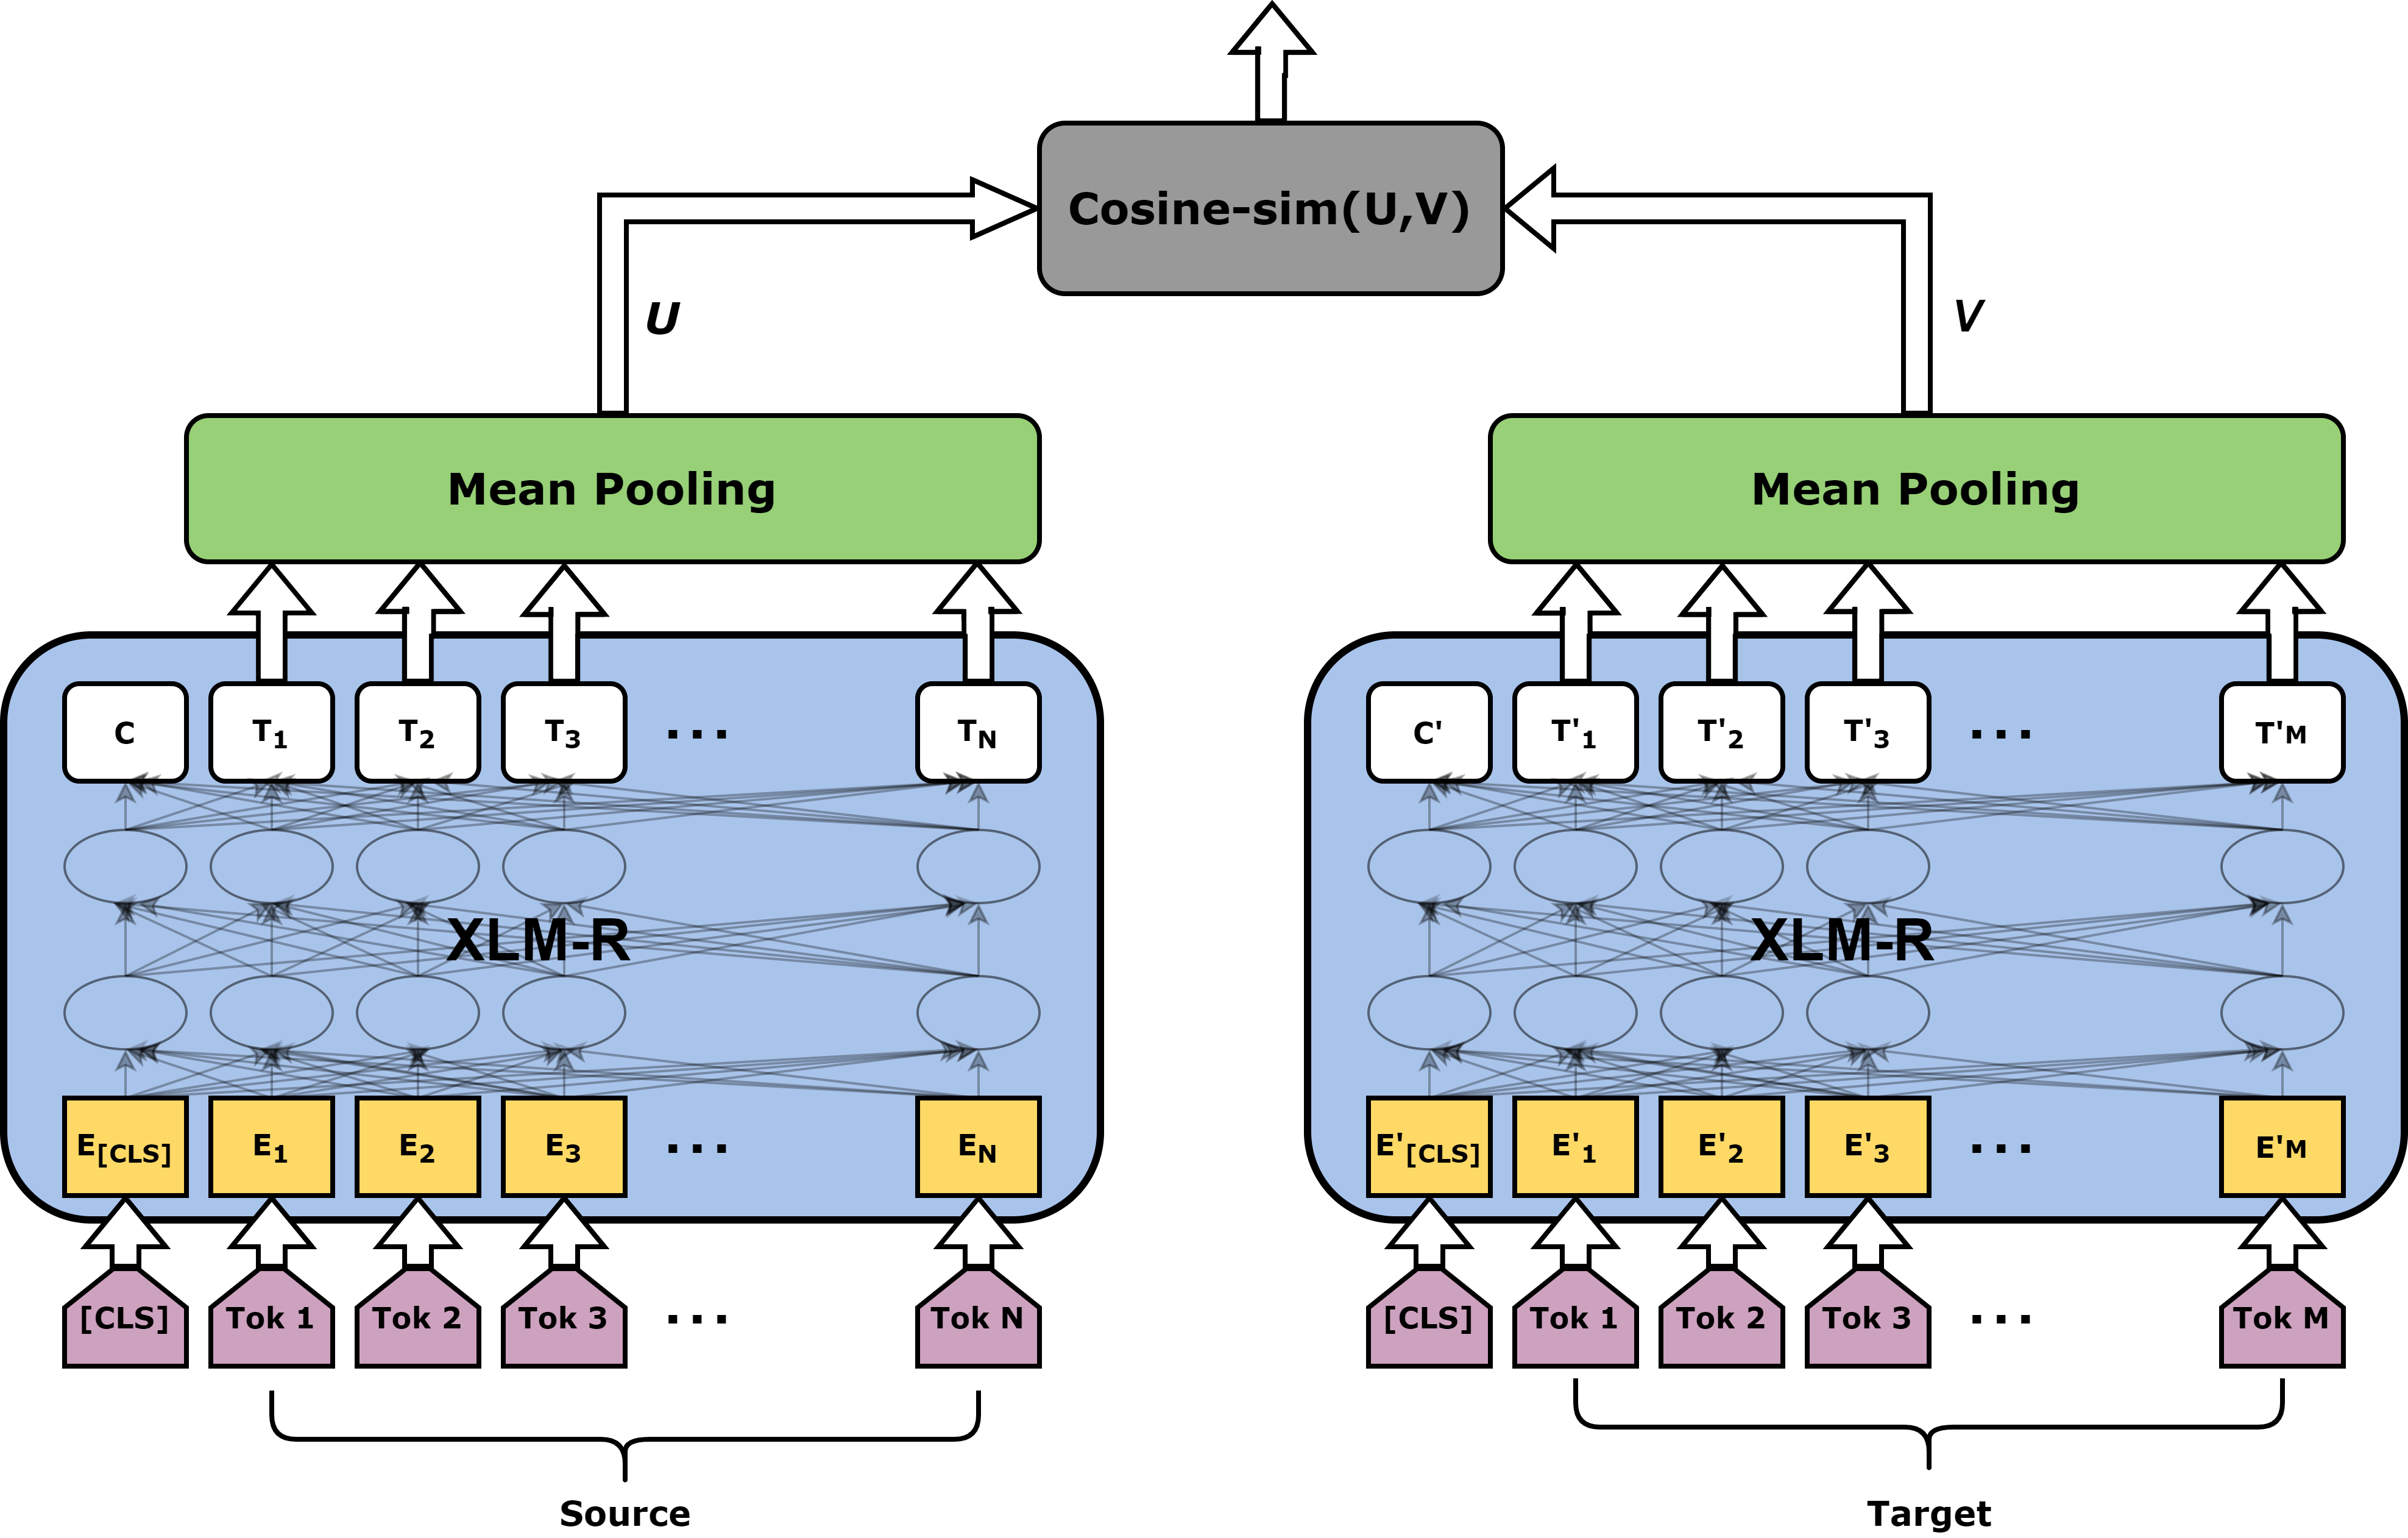
\includegraphics[width=12cm]{figures/translation_quality_estimation/SiameseTransQuest.png}
		\caption{\textit{SiameseTransQuest} Architecture}
		\label{fig:siamesetransquest}
	\end{subfigure}
	
	\caption{Architecture in TransQuest}
	\label{fig:architecture}
\end{figure}


\section{Results and Evaluation}


\renewcommand{\arraystretch}{1.2}
\begin{table}[t]
	\begin{center}
		\small
		% \footnotesize
		\scalebox{0.8}{
		\begin{tabular}{l l  c c c c c c c c} 
			%\hline
			\toprule
			& & \multicolumn{4}{c}{\bf Mid-resource} & \multicolumn{4}{c}{\bf High-resource}\\\cmidrule(r){3-6}\cmidrule(r){7-10}
			&{\bf Method} & \makecell{En-Cs \\ SMT} & \makecell{ En-Ru \\ NMT} & \makecell{En-Lv \\ SMT} & \makecell{En-Lv \\ NMT} & \makecell{De-En \\ SMT} & \makecell{En-Zh \\ NMT} & \makecell{En-De \\ SMT } & \makecell{En-De \\ NMT} \\
			\midrule
			\multirow{2}{*}{\bf I} & MTransQuest & \textbf{0.7207} & \textbf{0.7126} & 0.6592 & 0.7394 & \textbf{0.7939} & 0.6119 & 0.7137 & \textbf{0.5994}\\
			& STransQuest & 0.6853 & 0.6723 & 0.6320 & 0.7183 & 0.7524 & 0.5821& 0.6992 & 0.5875 \\
			\midrule
			\multirow{2}{*}{\bf II} & MTransQuest *-En$|$En-* & 0.7168 & 0.7046  & \textbf{0.7181} & \textbf{0.7482} & 0.7939 & 0.6101 & 0.7355 & 0.5992 \\
			& STransQuest *-En$|$En-* & 0.6663 & 0.6701 & 0.6533 & 0.7192 & 0.7524 & 0.5721 & 0.7000 & 0.5793 \\
			\midrule
			\multirow{2}{*}{\bf III} & MTransQuest-m & 0.7111 & 0.7012 & 0.7141 & 0.7450 & 0.7878 & 0.6092 & 0.7300 & 0.5982 \\
			& STransQuest-m & 0.6561 & 0.6614 & 0.6621 & 0.7202 & 0.7369 & 0.5612 & 0.7015 & 0.5771 \\
			%\midrule
			\midrule
			\multirow{3}{*}{\bf IV} & Quest ++ & 0.3943 & 0.2601 & 0.3528 & 0.4435 & 0.3323 & NR & 0.3653 & NR \\
			& OpenKiwi & NR & 0.5923 & NR & NR & NR & 0.5058 & 0.7108 & 0.4001 \\
			& Best system & 0.6918 & 0.5923 & 0.6188 & 0.6819 & 0.7888 & \textbf{0.6641} & \textbf{0.7397} &  0.5718 \\
			\midrule
			\multirow{1}{*}{\bf V} & mBERT & 0.6423 & 0.6354 & 0.5772 & 0.6531 & 0.7005 & 0.5483 & 0.6239 & 0.5002 \\
			\bottomrule
			%\bottomrule
		\end{tabular}
	}
	\end{center}
	\caption[Pearson correlation between TransQuest algorithm predictions and human post-editing effort]{Pearson ($r$) correlation between \textit{TransQuest} algorithm predictions and human post-editing effort. Best results for each language by any method are marked in bold. Rows I, II and III indicate the different evaluation settings. Row IV shows the results of the state-of-the-art methods and the best system submitted for the language pair in that competition. \textbf{NR} implies that a particular result 
		% from a state-of-the-art method 
		was \textit{not reported} by the organisers. Row V presents the results of the multilingual BERT (mBERT) model in MonoTransQuest Architecture.} 
	\label{tab:hter_prediction}
\end{table}
\section{Conclusion}